\documentclass[11pt]{article}

\usepackage[margin=1in]{geometry}
\usepackage{graphicx}
\usepackage[hidelinks]{hyperref}
\graphicspath{{figures/}}
\renewcommand{\familydefault}{\sfdefault}
\setlength{\parindent}{0pt}
\pagestyle{plain}

\title{Supplementary Information\\[4pt]
\large When does ESM3 fuse its modalities? A geometry-first atlas of the
multimodal residual stream}
\author{Jacob L. Steenwyk}
\date{}

\begin{document}
\maketitle
\thispagestyle{plain}
\vspace{1em}
This document contains supplementary Figures S1 to S10. Each figure supports, but does
not lead, a result in the main text.
\clearpage

\begin{center}
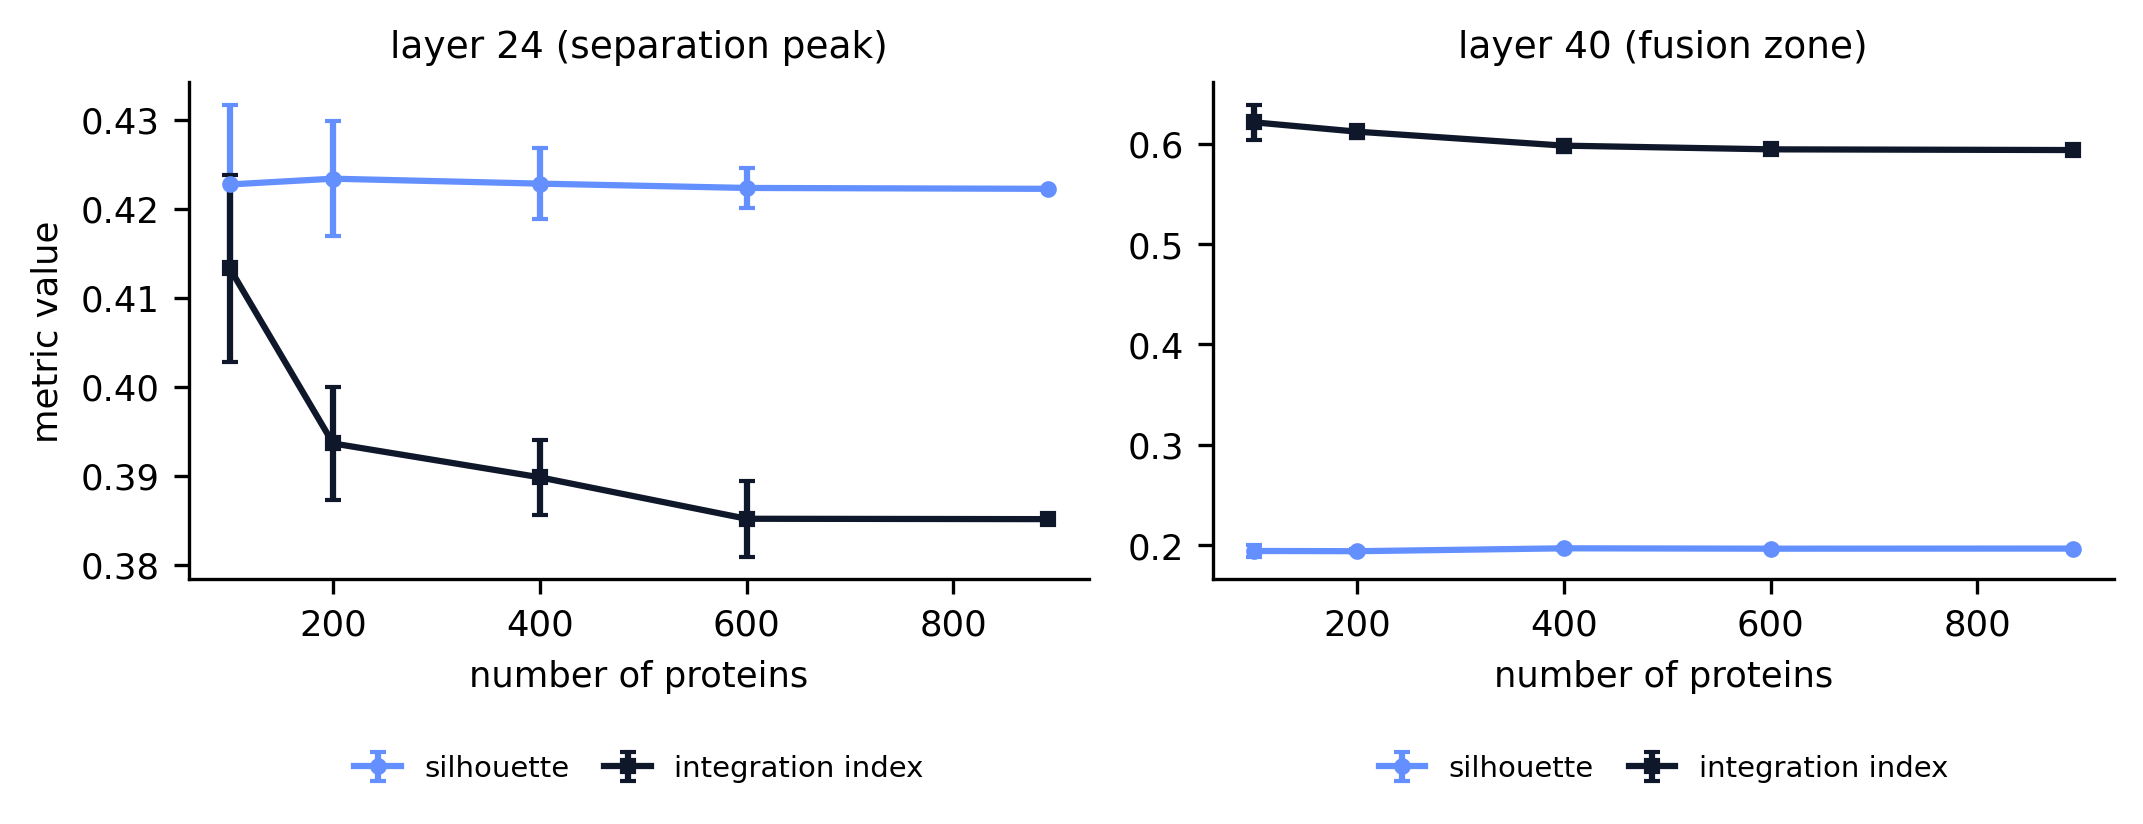
\includegraphics[width=\linewidth,height=0.74\textheight,keepaspectratio]{figureS1.png}
\end{center}
\vspace{0.6em}
{\small\textbf{Figure S1. The metrics are converged at the sample size used.} Silhouette and integration index computed on random subsamples of the 892-protein set (mean and standard deviation over 12 draws per size) at layer 24 (separation peak) and layer 40 (fusion zone). Silhouette is stable from 100 proteins, and the integration index settles by 400 to 600 proteins, so 892 proteins lie within the converged regime for every reported quantity.}
\clearpage
\begin{center}
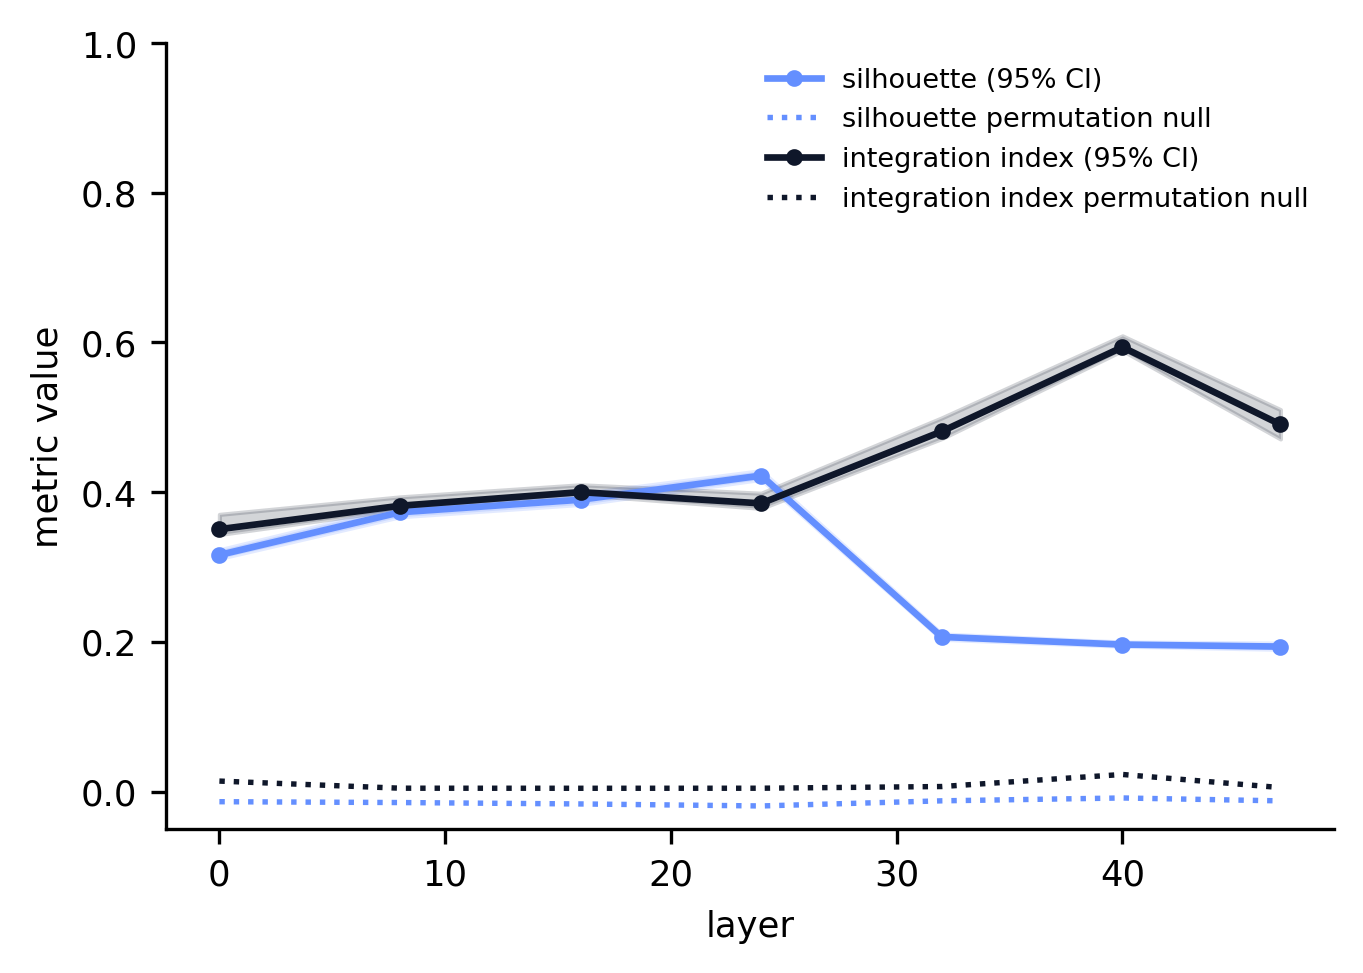
\includegraphics[width=\linewidth,height=0.74\textheight,keepaspectratio]{figureS2.png}
\end{center}
\vspace{0.6em}
{\small\textbf{Figure S2. Every fusion metric is significant against a permutation null.} For the canonical layers, the observed silhouette and integration index (points, with protein-bootstrap 95 percent confidence bands) sit far above their label-permutation null means (dotted), with permutation p of 0.005 at every layer tested.}
\clearpage
\begin{center}
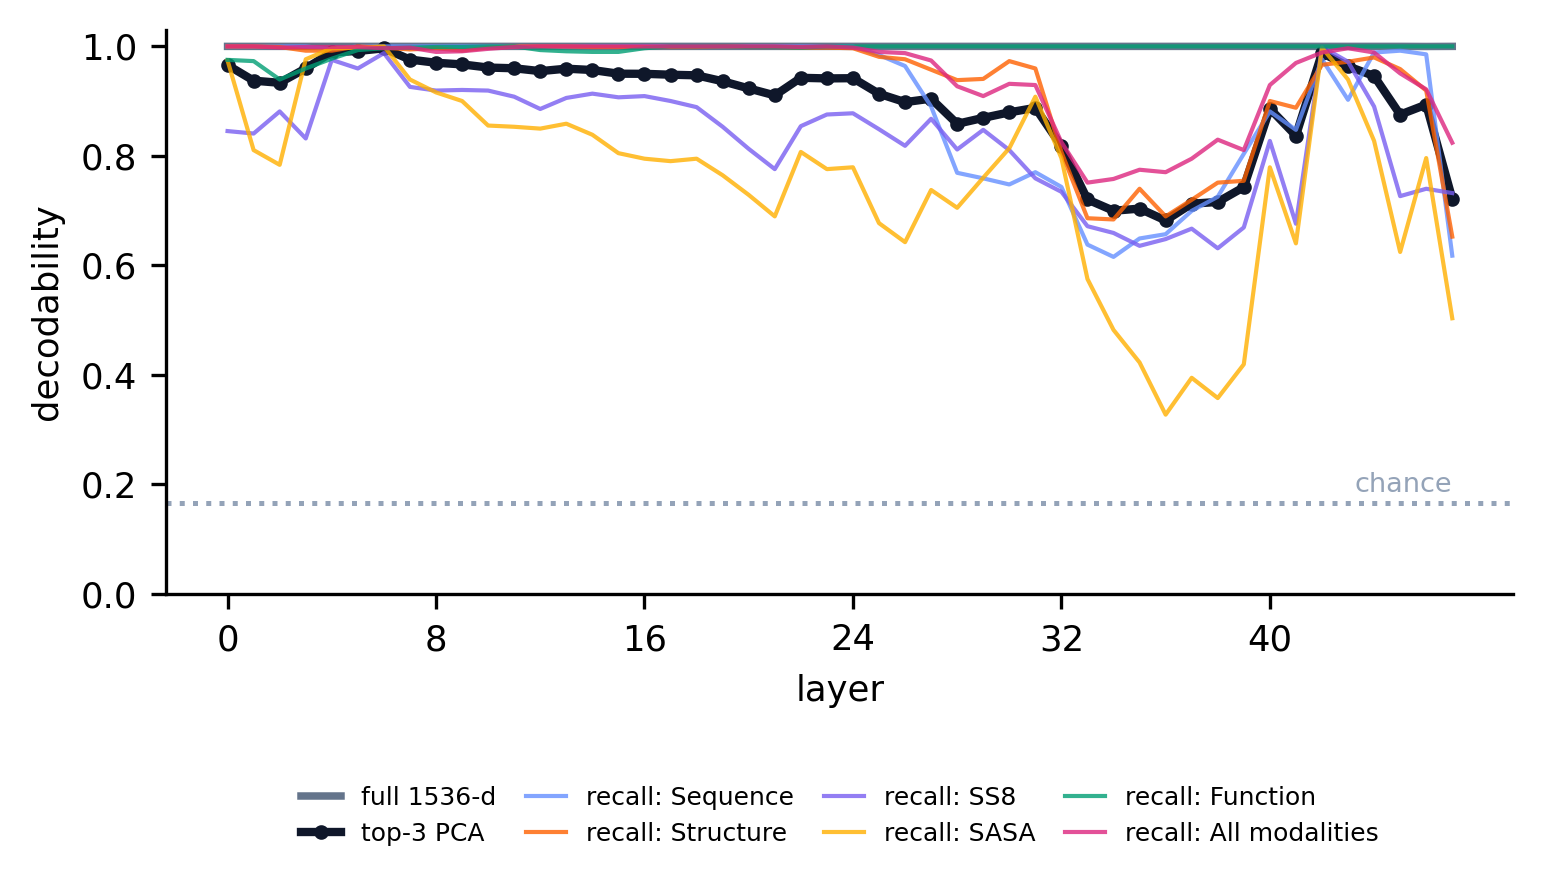
\includegraphics[width=\linewidth,height=0.74\textheight,keepaspectratio]{figureS3.png}
\end{center}
\vspace{0.6em}
{\small\textbf{Figure S3. Modality identity stays decodable, and the functional channel stays decodable longest.} A protein-grouped logistic probe of modality identity. In the full 1536-dimensional stream, decodability is 1.0 at every layer (an additive modality tag persists). In the top-3 PCA geometry, overall accuracy falls to about 0.68 in the fusion zone, driven by SASA (per-condition recall near 0.33), whereas the function condition stays near 1.0 throughout. Chance is 1 of 6.}
\clearpage
\begin{center}
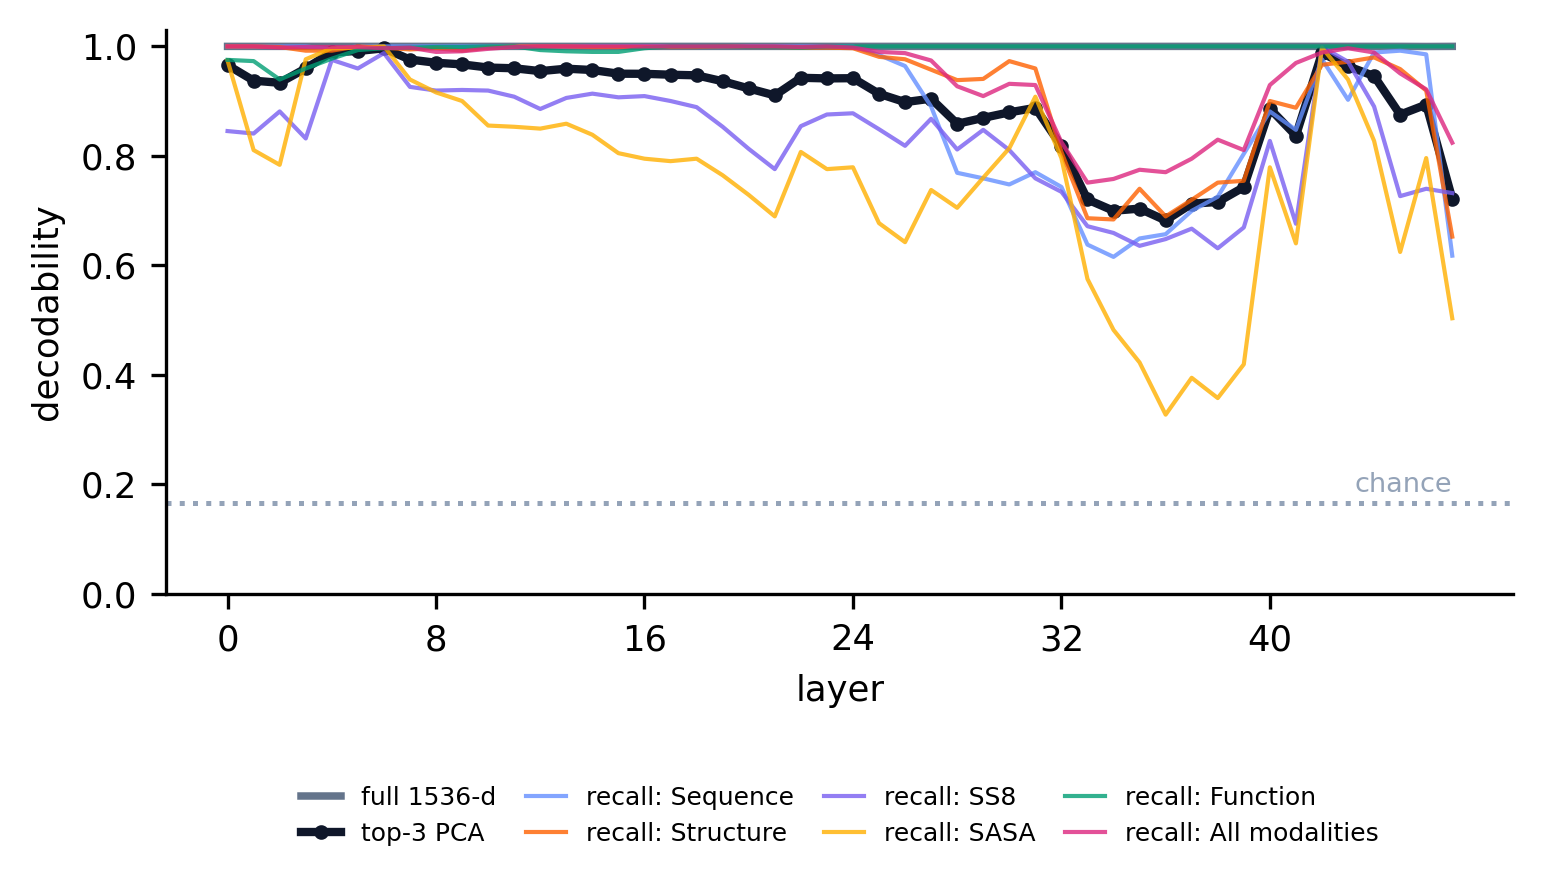
\includegraphics[width=\linewidth,height=0.74\textheight,keepaspectratio]{figureS4.png}
\end{center}
\vspace{0.6em}
{\small\textbf{Figure S4. Every individual organism reaches peak fusion at the same depth.} Condition separation across depth for each of the 12 organisms (thin lines, coloured by superkingdom) and for the pooled set (thick line). All 12 organism curves and the pooled curve reach minimum separation at layer 35 (dotted line).}
\clearpage
\begin{center}
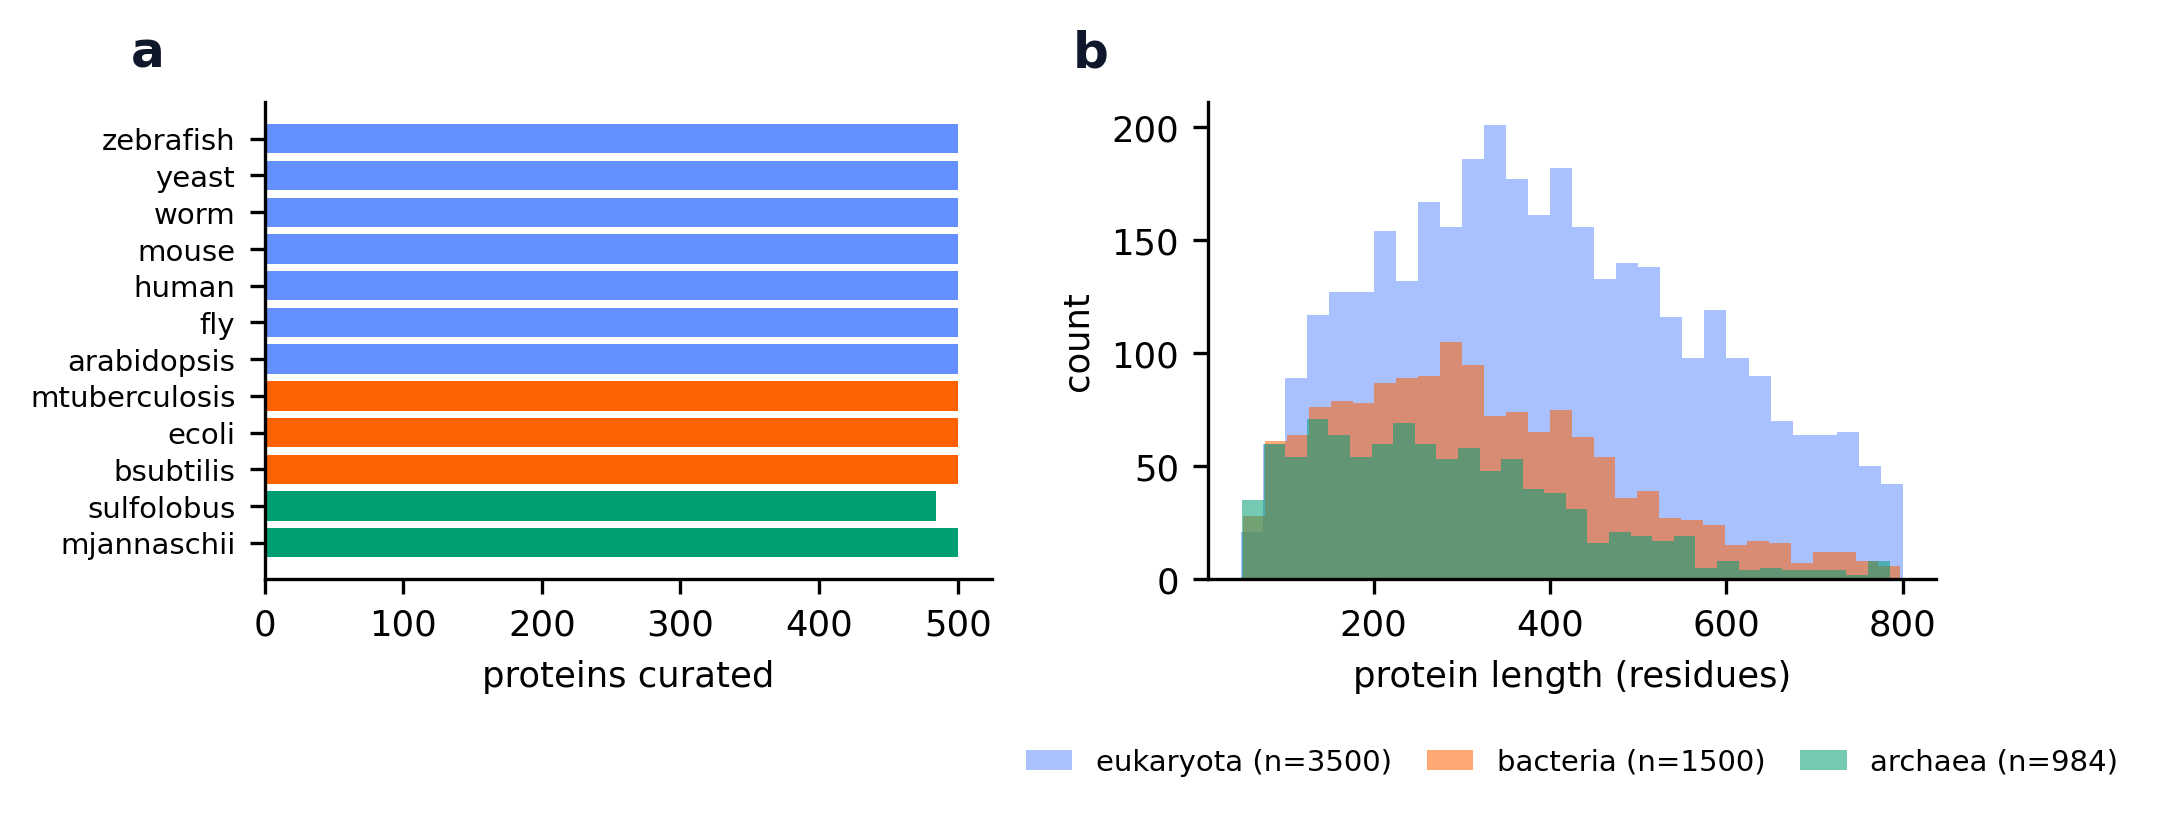
\includegraphics[width=\linewidth,height=0.74\textheight,keepaspectratio]{figureS5.png}
\end{center}
\vspace{0.6em}
{\small\textbf{Figure S5. The condition-by-condition CKA matrix warms with depth except along the function axis.} Linear CKA between all six conditions at seven depths. The structure, SS8, and SASA block is warm from layer 0, the sequence entries warm after layer 24, and the function row and column stay near CKA 0 at every depth.}
\clearpage
\begin{center}
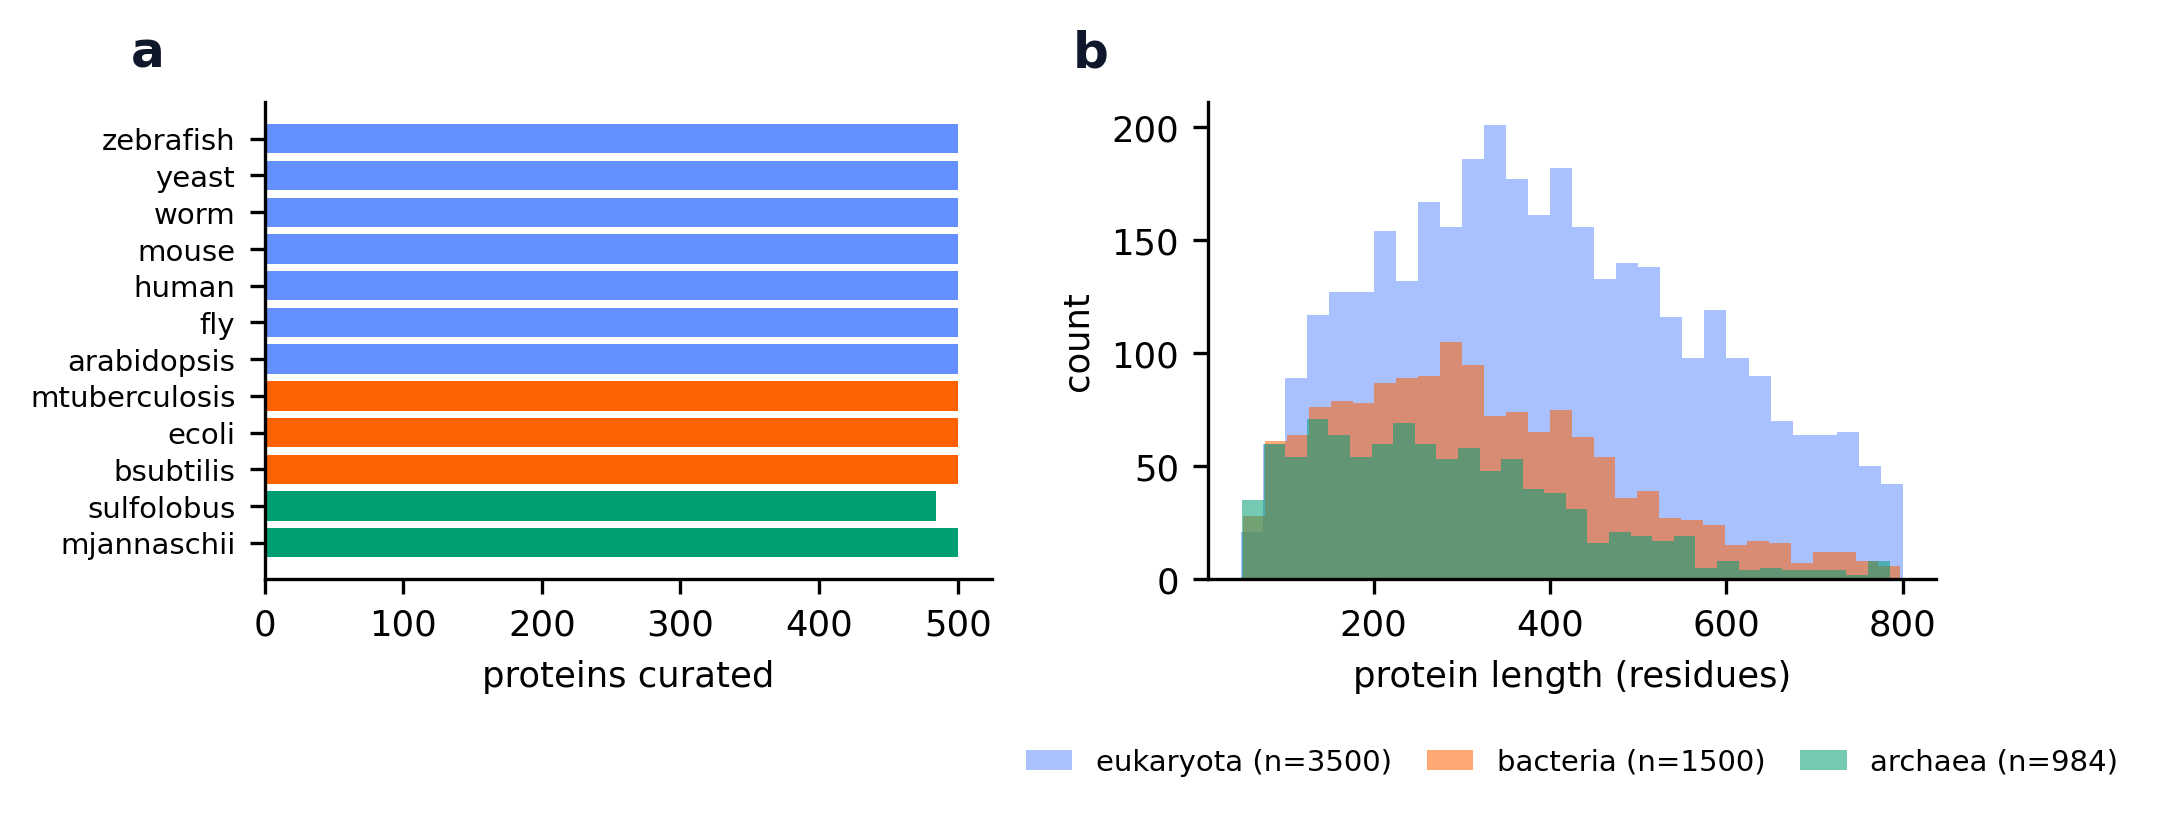
\includegraphics[width=\linewidth,height=0.74\textheight,keepaspectratio]{figureS6.png}
\end{center}
\vspace{0.6em}
{\small\textbf{Figure S6. Composition of the 12-organism diverse set.} (a) Proteins curated per organism (about 500 each), coloured by superkingdom. (b) Protein-length distributions by superkingdom over the 50 to 800 residue range.}
\clearpage
\begin{center}
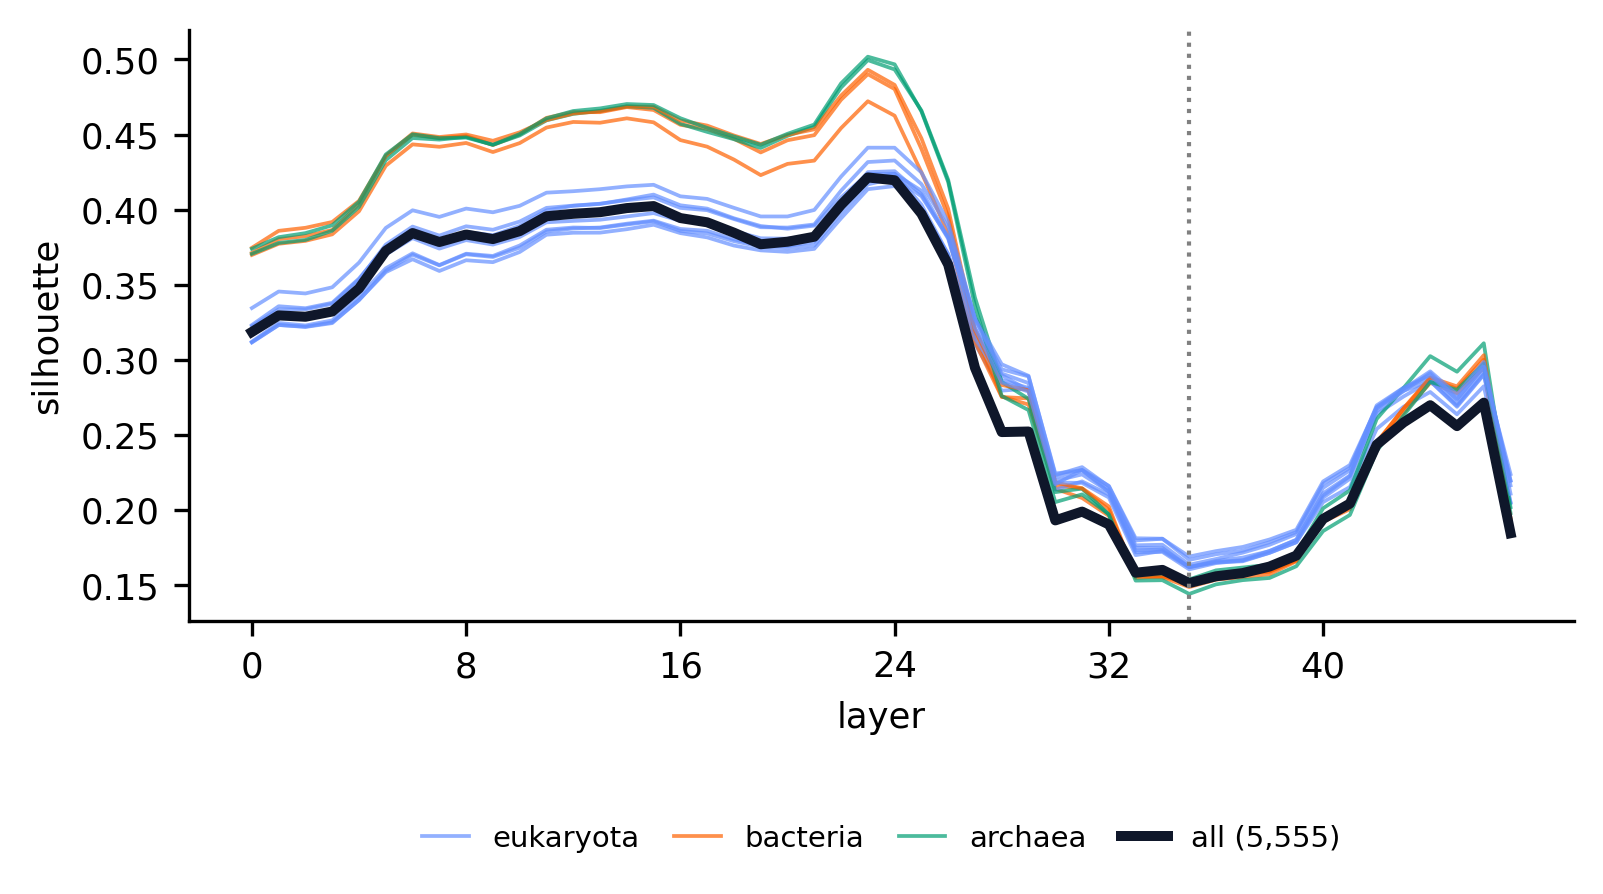
\includegraphics[width=\linewidth,height=0.74\textheight,keepaspectratio]{figureS7.png}
\end{center}
\vspace{0.6em}
{\small\textbf{Figure S7. The representation is organised by modality, not by source organism.} (a) The layer-40 all-modalities representation of 5,555 proteins, projected to three dimensions and coloured by superkingdom. Eukaryota, bacteria, and archaea are intermixed rather than separated. (b) Across depth, condition separation by modality (silhouette, reaching 0.42 at layer 24) far exceeds separation by superkingdom, which stays near 0 at every layer (peaking at only 0.08 at layer 33). ESM3 therefore represents proteins by their biochemistry rather than their taxonomy.}
\clearpage
\begin{center}
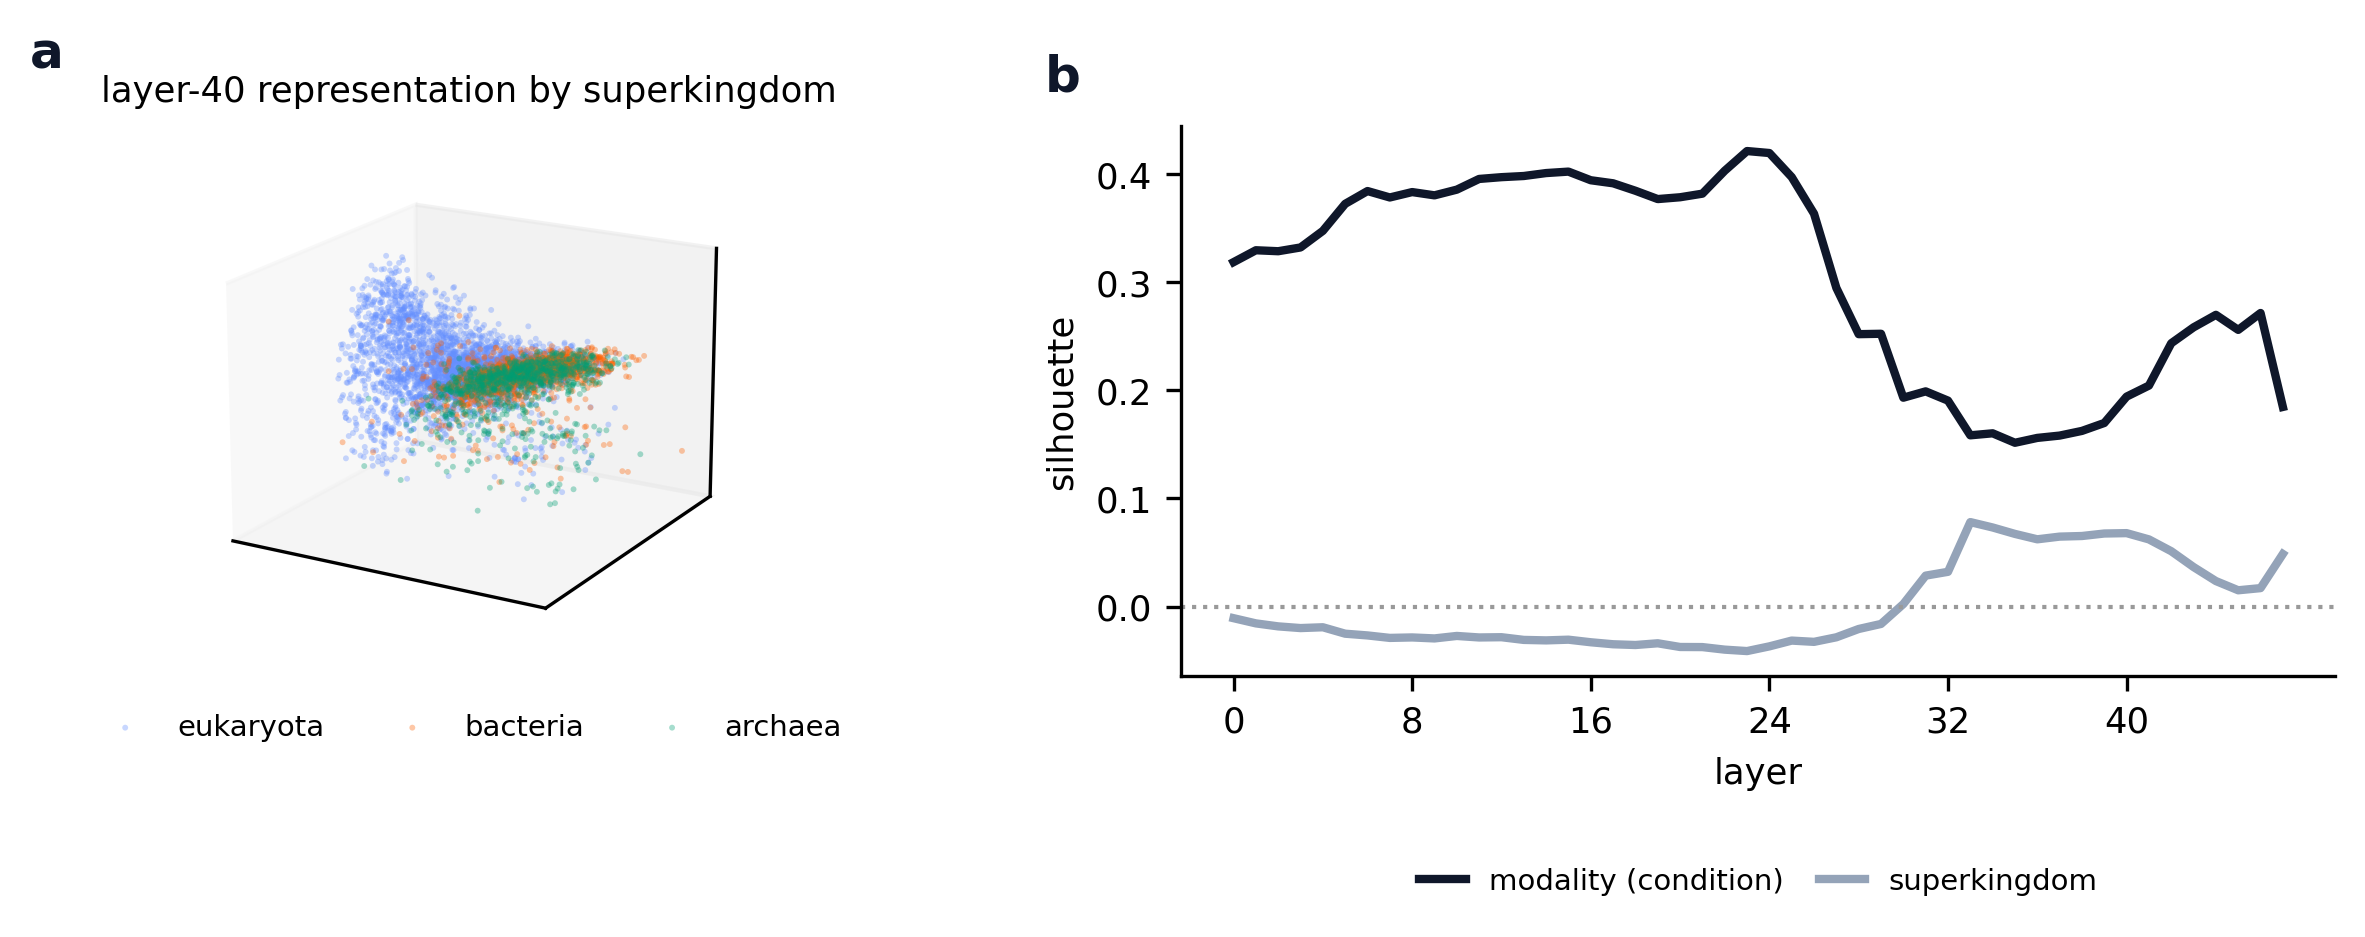
\includegraphics[width=\linewidth,height=0.74\textheight,keepaspectratio]{figureS8.png}
\end{center}
\vspace{0.6em}
{\small\textbf{Figure S8. Function orthogonality does not reflect redundancy.} Per-protein alignment is the cosine between a protein's function vector and its mean physical vector, averaged over layers 32, 40, and 47, after centring each condition. If function stayed orthogonal only because it is recoverable from the physical modalities, alignment should be higher for proteins whose function is not recoverable. (a) Proteins split by whether the structure-derived representation correctly decodes enzyme class. The non-redundant group, for which structure fails, aligns no more than the redundant group (medians near 0, Mann-Whitney p = 0.35). (b) Alignment against InterPro domain count shows no trend (Spearman r = -0.02). Alignment is near zero for every protein regardless of redundancy, which favours a categorical account of the functional channel over a redundancy account.}
\clearpage
\begin{center}
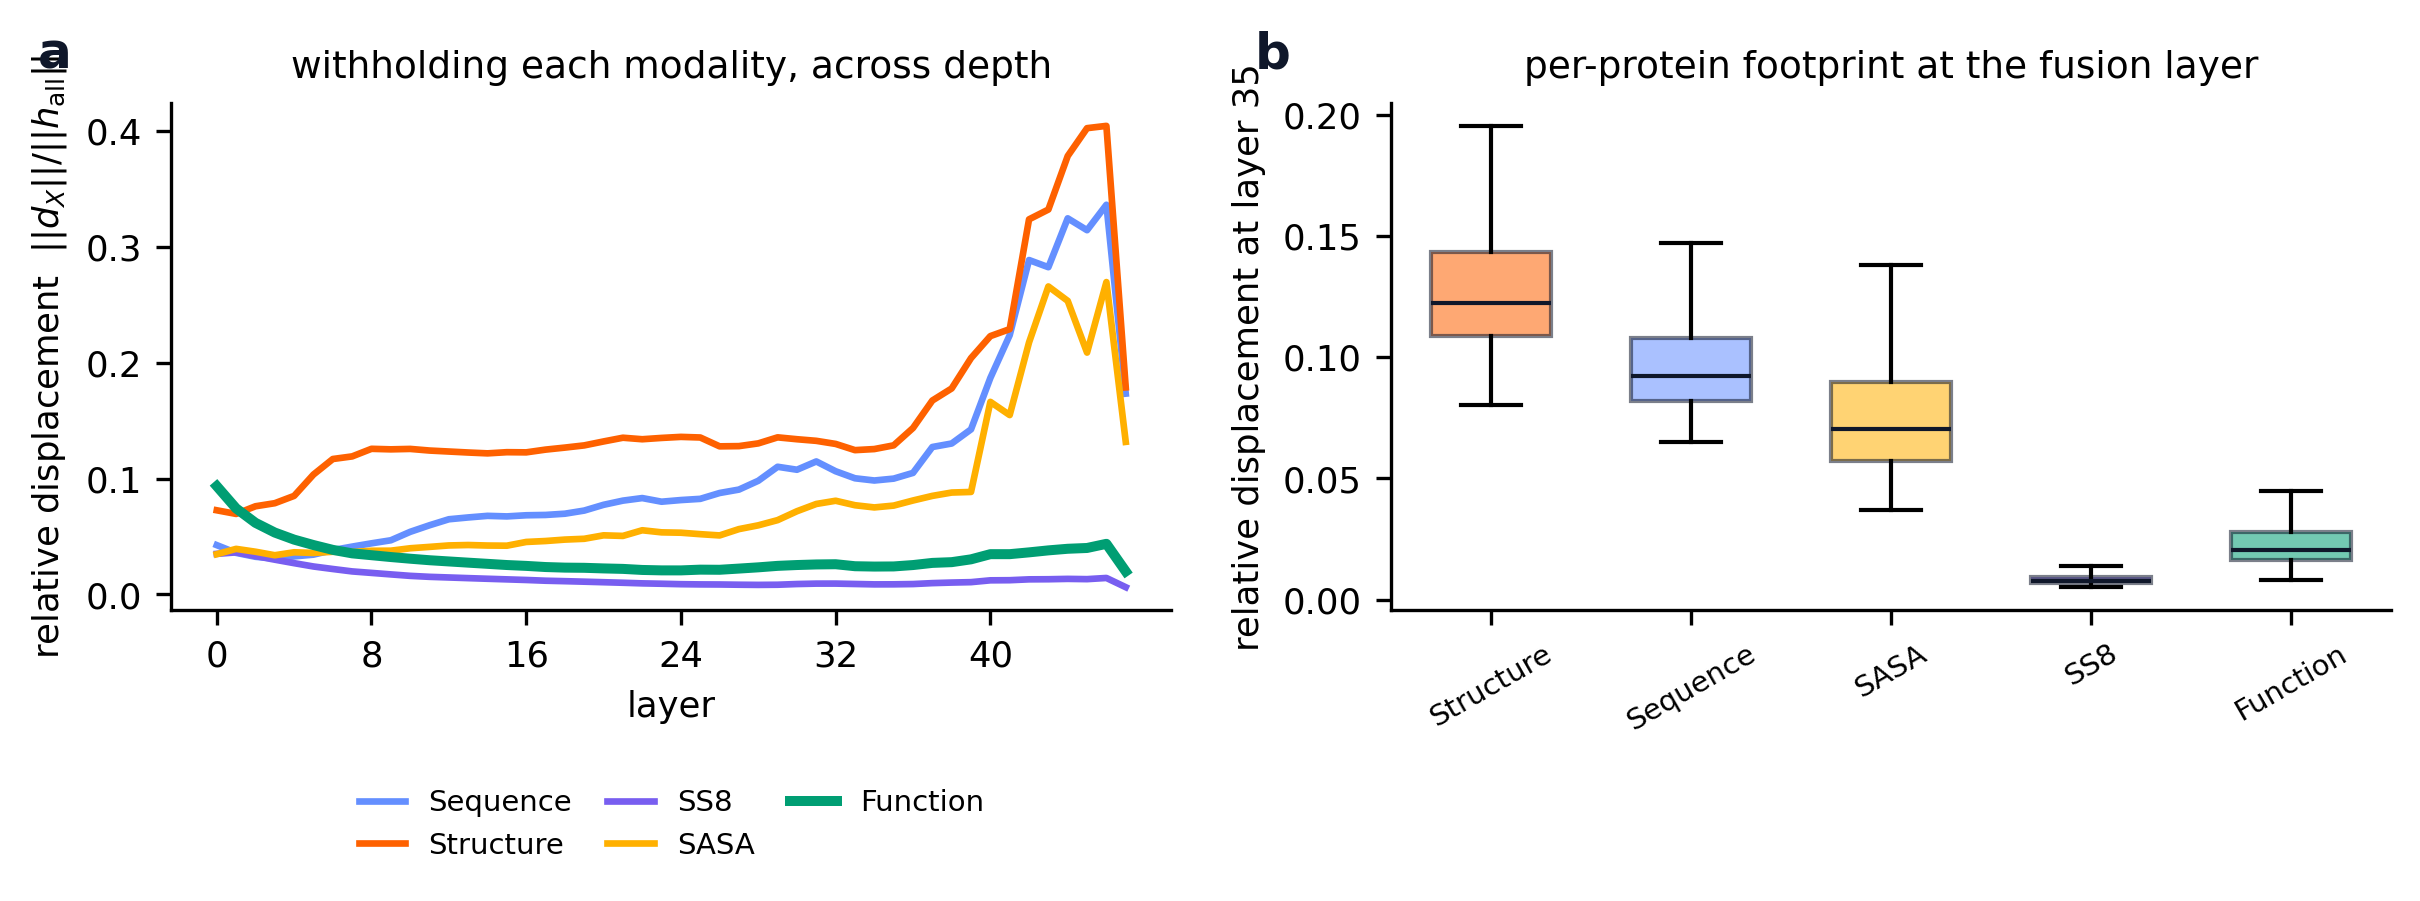
\includegraphics[width=\linewidth,height=0.74\textheight,keepaspectratio]{figureS9.png}
\end{center}
\vspace{0.6em}
{\small\textbf{Figure S9. Function content lives in the physical subspace even though the function channel is geometrically orthogonal.} A probe (standardisation, 50-component PCA, logistic regression, five-fold balanced accuracy) decodes a structural target (fold class from SS8, three classes) and a functional target (EC enzyme class, three classes) from each modality condition. (a) At the post-fusion layer 39 the physical conditions decode both targets well, whereas the function channel decodes both weakly, so there is no division of representational labour. (b) Across depth, enzyme class becomes more decodable from the structure-derived representation, reaching about 0.79, while the function channel decodes fold class near 0.40 and enzyme class near 0.55. Functional information is therefore present in the physical subspace, and the geometric orthogonality of the function channel reflects how the network organises the representation rather than an absence of functional content. The dotted line marks the chance rate of 0.33.}
\clearpage
\begin{center}
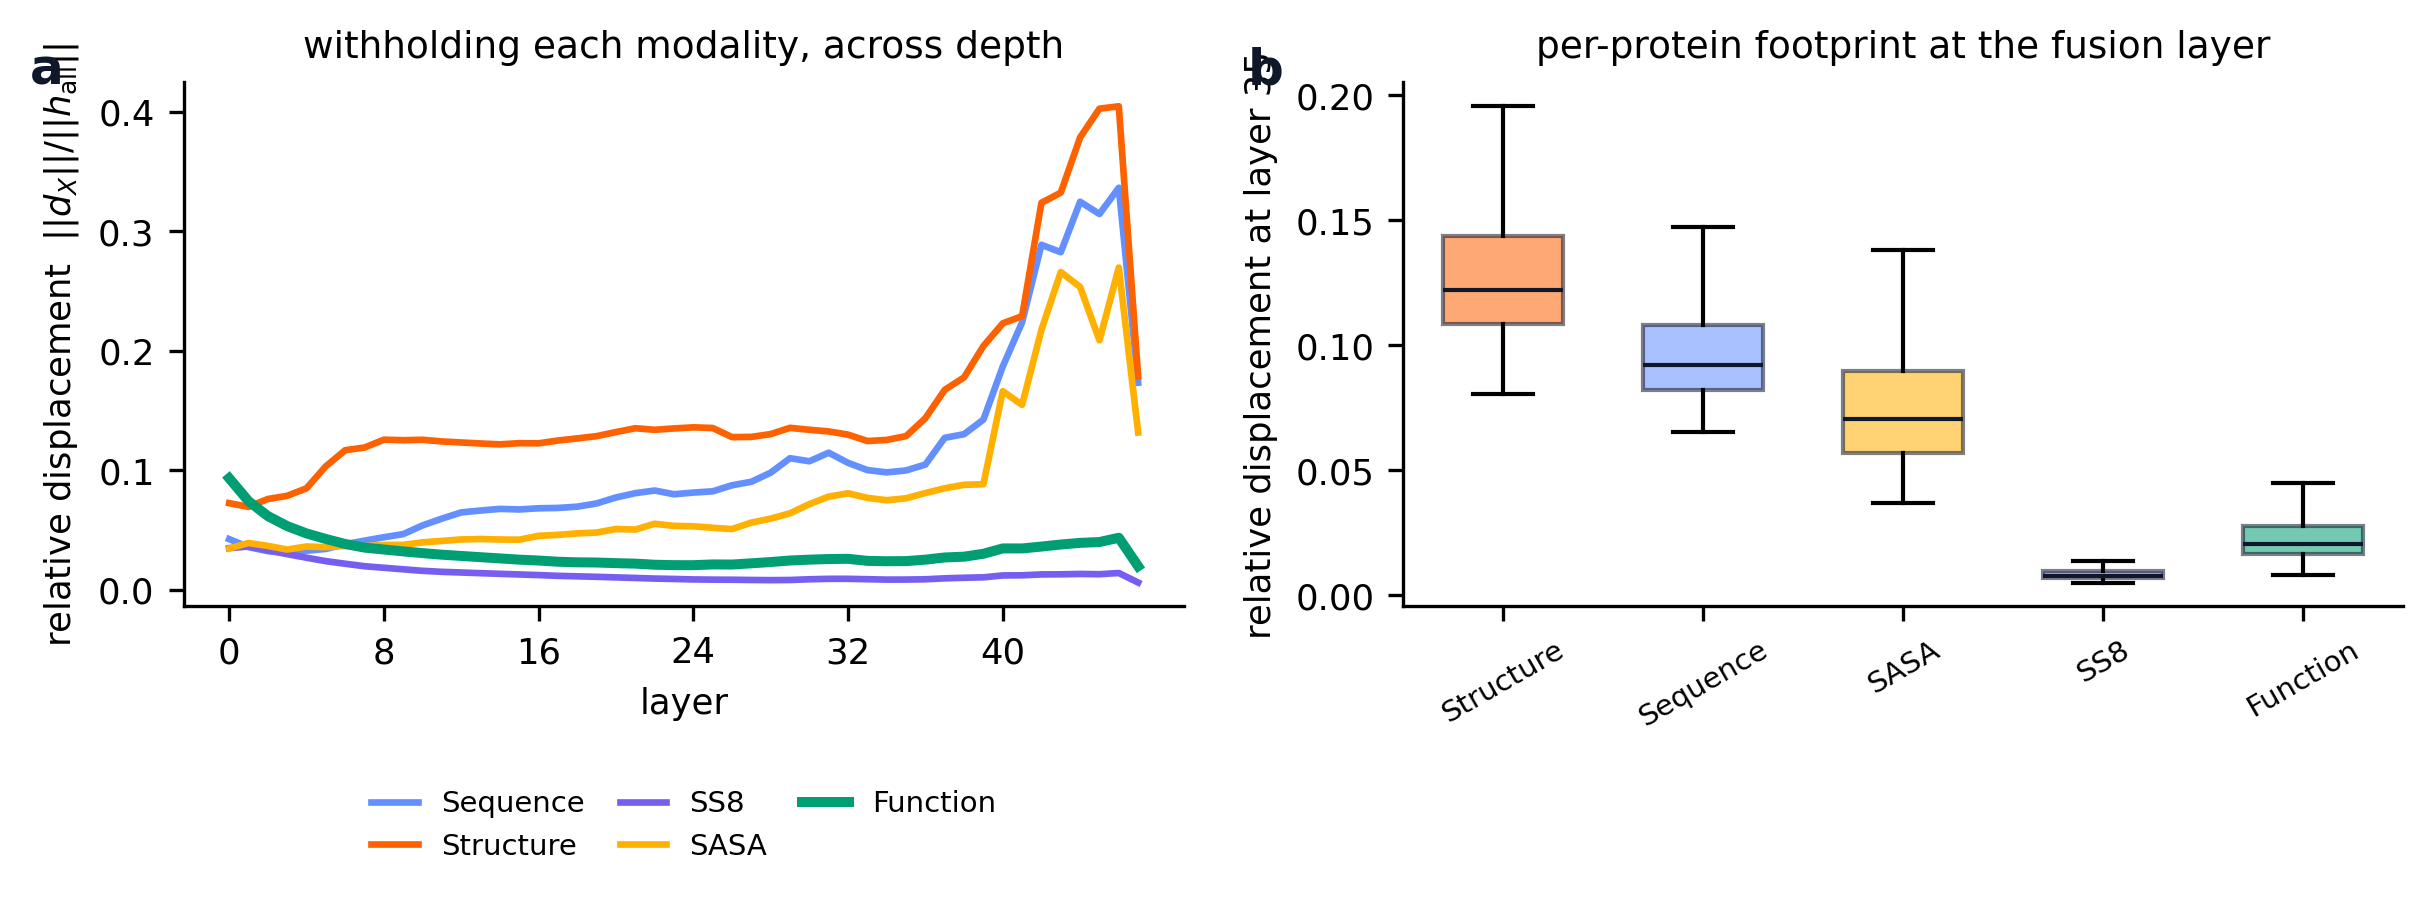
\includegraphics[width=\linewidth,height=0.74\textheight,keepaspectratio]{figureS10.png}
\end{center}
\vspace{0.6em}
{\small\textbf{Figure S10. Withholding function barely perturbs the fused representation.} Each modality's contribution is the displacement between the all-modalities representation and the representation with that modality withheld, measured for all 892 proteins as a fraction of the all-modalities vector norm. (a) Relative displacement across depth. Withholding function (green) moves the representation far less than withholding structure, sequence, or SASA, and the gap widens with depth. (b) Per-protein relative displacement at the fusion layer 35. The function footprint, with a median of 0.021, is about six times smaller than the structure footprint, with a median of 0.12. The ss8 footprint is smaller still, but because ss8 is redundant with structure rather than orthogonal, so a small footprint marks low marginal impact, which the geometric and decoding results attribute to orthogonality in the case of function. This is causal evidence that the fused physical representation is largely insensitive to the function input.}
\clearpage
\end{document}
